\documentclass[conference]{IEEEtran}
\usepackage{cite}
\usepackage{amsmath,amssymb,amsfonts}
% \usepackage{algorithmic}
\usepackage{graphicx}
\usepackage{textcomp}
\usepackage{xcolor}
\usepackage{fancyhdr}
\usepackage{algorithm}
\usepackage{algpseudocode}
\usepackage[hyphens]{url}

\def\BibTeX{{\rm B\kern-.05em{\sc i\kern-.025em b}\kern-.08em
    T\kern-.1667em\lower.7ex\hbox{E}\kern-.125emX}}

% Ensure letter paper
\pdfpagewidth=8.5in
\pdfpageheight=11in


\fancypagestyle{firstpage}{
  \fancyhf{}
\renewcommand{\headrulewidth}{0pt}
  \fancyhead[C]{CSE240A} 
  \fancyfoot[C]{\thepage}
}  


\pagenumbering{arabic}

%%%%%%%%%%%---SETME-----%%%%%%%%%%%%%
\title{Branch Predictor Project Report} 
\author{Pisit Wajanasara\\
PID: A59009987\\
University of California, San Diego}
%%%%%%%%%%%%%%%%%%%%%%%%%%%%%%%%%%%%

\begin{document}
\maketitle
\thispagestyle{firstpage}
\pagestyle{plain}



%%%%%% -- PAPER CONTENT STARTS-- %%%%%%%%

\begin{abstract}

Branch instructions are part of modern computer programs in today world and are known to decrease
the pipeline speed. To solve this problem, branch speculation was studied and various branch predictors
were created to reduce the branch misprediction rate. In the early era, there are some predictors such as
GShare, which can handle the global branch correlation, or the tournament predictor, which is composed
of multi predictors and can handle both local and global branch correlation. In this work, we proposed
a branch predictor based on the tournament predictor with some modification. Our result showed that
it can beat both GShare and the tournament predictor for all testing traces in the term of misprediction rate.

\end{abstract}

\section{Introduction}

Real-world Computer programs consist of considerable amount of branch instructions. Without any branch speculation,
the pipeline can be slowed down since it need to flush the pipeline in the case that fetched instructions were wrong \cite{bp_survey1}.
To boost the pipeline performance, modern computer archiectures increasingly rely on branch speculation in order
to predict whether the branch will be taken or not \cite{perceptron_predictor}. With more prediction accuracy, the pipeline can gain more performance.

The branch predictor is designed as a component which receive branch instruction address as its inputs. After processing,
the branch predictor will output a bit to determine whether the given branch will be taken or not. One of the most
advantage of the branch predictor is to reduce number of pipeline flush which improve the processor performance. However,
designing the branch predictor come with limitations. The implemented component need to be inside the processor chip.
Thus, the storage for storing branch predictor information is limited. The speed of the branch predictor need to be fast
so that it doesn't slow down pipeline stages.

Branch prediction has been studied and developed for decades. An earlier version of branch prediction
might just used the saturating counter for each branch address to determine the branch outcome.
Many improvements had been done during the past time. One of the improvement was GShare predictor which can handle
the global correlation between branches. Later, there is another idea to combine the local branch predictor and the global
branch predictor together with another component to choose the appropriate predictor for different
addresses. The very first implementation of this idea is in Alpha 21264 processor \cite{Alpha21264} which shown a very good performance
in our benchmark.

In this project, we proposed another branch predictor based on the tournament predictor. We looked at how the tournament predictor
behaved and its problems. We ended up by modify some components of the predictor to increase more prediction
accuracy on our testing traces. The objective of our predictor is to perform better than provided GShare and
the tournament predictor baselines.

\section{Background}

In this section, we described two different branch predictors which we used as our baselines;
1) GShare and 2) Tournament predictor.

\begin{enumerate}
  \item GShare

  The branch outcomes are not only depend on the local history of the considering
  branches. Sometimes, it also depends on outcome from other branches. This correlation
  is called global correlation. This is done by having a global history register (GHR) which
  tracks all outcomes from all branches. To make a prediction, GShare uses xoring result
  between GHR and address in the program counter as an index to the 2-bit states prediction table. 
  The advantage of this predictor is to handle the global correlation between branch histories and
  current branch address which can't be done in the earlier predictor. However, there is also some
  cons. For example, it can lose the local branch correlation and the misprediction rate
  could be higher.

  \item Tournament predictor

  The tournament predictor is used in the Alpha 21264 processor \cite{Alpha21264}. Instead of using only one predictor,
  this predictor is a combination of multiple predictors. In Alpha 21264, there are two predictors for
  global and local prediction. The global predictor use information from GHR to select the prediction state
  in the prediction state table. The local predictor is a 2-level predictor which has the local branch history
  in the first level and the prediction state table in the second level. In order the choose the appropriate
  predictor for an input branch address, This predictor use another component to learn and choose the predictor
  for each prediction. The advantage of this predictor is that it can handle both global and local branch correlation.
  Anyway, this come with a trade-off. Using two predictors requires large storage, so we need to reduce the size of
  both local and global predictor to fit in the budget storage.

\end{enumerate}

\section{Design Ideas}

Our design is based mostly on tournament branch predictor used in Alpha 21264's branch
predictor.

In the tournament branch predictor, it used both local and global branch prediction
with a choice prediction to choose the right predictor for different branches.
This help the predictor to handle both local and global correlation between branches.
In this work, we also utilize this idea and we decided to improve both local and global
branch prediction method in our custom predictor.

First, we decided to look at the global predictor. If we compare between Alpha 21264's
global predictor and GShare, we will notice that the index hashing schemes are different.
For GShare, it used $index = (pc \oplus GHR) \mod{n}$ to index the global counter. While the latter
predictor used only $pc \mod{n}$ as the index. We believe that GShare's index is better
at incorporate both pc and GHR information to select the counter. In addition, we have more
storage for storing the data for branch predictor. Thus, we decided to increase the size of
global predictor too.

Secondly, for the local branch predictor, we observed that the implementaion in the
Alpha 21264's predictor performed very well with 2-bit saturating counter. Thus, we decided
to keep the counter as is. However, to efficiently use the increase storage size, we increased
the size of the local history table instead.

The predictor chooser in the Alpha 21264's worked fine. However, we thought that the hashing
index should be changed. Instead of indexing the chooser by the global history register,
we changed the index to be the program counter instead. Thus, the chooser will select the
predictor based on the current instruction address instead of the global
history of the branch outcome.

\section{Implementation details}

In this section, we explained how our predictor was implemented. The proposed predictor is
based on Alpha 21264's branch predictor which include the local predictor, the global predictor
and the chooser as its components.

\subsection{Overall Design}

The overview design of our predictor is shown in Figure \ref{fig:overall_design}. We have two different
predictors inside the our predictor targeting global correlation and local correlation predictions.
One thing to notice is that global predictor is using the xor result between the global history register
and the program counter as the index. However, for the the rest of the components, we used only program
counter for indexing.

During the prediction process, both predictors will give a prediction output, but only one prediction
will be chosen by the predictor chooser. We incorporate a mux here as a selector. The output from the mux
is the prediction result from our predictor.

After each prediction was done and the real branch outcome was revealed, the predictor need to be updated.
Both local and global predictor are both updated at the same time with new information which we will describe
the update process later in this report. The predictor chooser is also updated in this state. After all
components are updated, we update the global history register to include the new outcome to our history.
This is done by left shifting the global history register, then the new outcome is added to its last bit.


\begin{figure}[h]
    \centering
    % \vspace{0.2cm}
    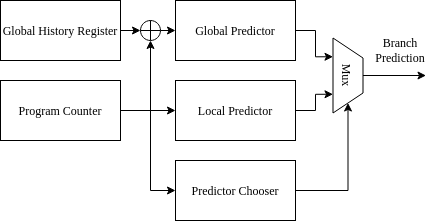
\includegraphics[width=0.45\textwidth]{imgs/overall_design}
    \caption{The overall design of the proposed branch predictor. We have 2 predictors including
    the local and the global predictor for capturing different local/global branch patterns. The
    global predictor is indexed by the xored result between the global history register and the program
    counter. The local predictor is indexed by the program counter only. The predictor chooser select
    the result from both predictor by looking at the current address in the program counter.}
    \label{fig:overall_design}
\end{figure}

\subsection{Local branch predictor}

The presented local branch predictor in our work is based from the implementation in the tournament
predictor. The n least significant bit from program counter is used to index the local history table.
After that, we get the local history from that table. This history is a bit vector of Taken (T/1) and Not-Taken
(N/0), which is used to index the local prediction table. The local prediction table will give the
prediction result based on the state in the table. In this work, we used 2-bit predictors as our
prediction table. This includes 4 possible states including strongly not-taken (SN/00),
weakly not-taken (WN,01), weakly taken (WT/10) and strongly taken (ST/11). The first two states
will give not-taken as the prediction result, while the last two will give taken as the prediction
result. The internal process of this predictor is also shown in Figure \ref{fig:local_predictor}.

\begin{figure}[h]
    \centering
    % \vspace{0.2cm}
    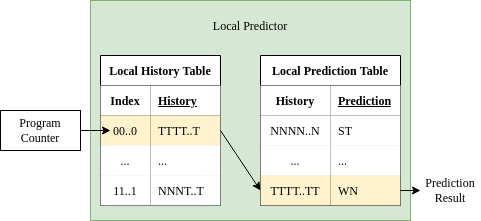
\includegraphics[width=0.48\textwidth]{imgs/local_predictor}
    \caption{The local predictor has two components. First component is the local history table with
    hold the mapping table from address index to local branch history. Then, the obtained branch history
    is used to get the prediction table state which determines the prediction result.}
    \label{fig:local_predictor}
\end{figure}

During the update phase, the history related to the instruction address is updated with the new outcome.
The prediction table state also get updated regarding the new branch outcome. We update the state toward
strongly not-taken and toward strongly taken when the outcome is not-taken and taken respectively.

% \begin{algorithm}
% \caption{An algorithm with caption}\label{alg:local_predictor_update}
% \begin{algorithmic}
% \Require $n \geq 0$
% \Ensure $y = x^n$
% \State $y \gets 1$
% \State $X \gets x$
% \State $N \gets n$
% \While{$N \neq 0$}
% \If{$N$ is even}
%     \State $X \gets X \times X$
%     \State $N \gets \frac{N}{2}$  \Comment{This is a comment}
% \ElsIf{$N$ is odd}
%     \State $y \gets y \times X$
%     \State $N \gets N - 1$
% \EndIf
% \EndWhile
% \end{algorithmic}
% \end{algorithm}


\subsection{Global branch predictor}

For the global branch predictor, we modified Alpha 21264's global predictor to use the GShare index
instead of just the global history register. The GShare index is calculated by xoring the global history
table with the address in the program counter. This help incorporate both information to select the right
prediction state for the global prediction, i.e., the same address with a different history will point to a
different row in the prediction table. Same as the local branch predictor, the global prediction table stores
2-bit states which related to strongly not-taken, weakly not-taken, weakly taken and strongly taken as described
in the previous section. The internal implementation of this component is shown in Figure \ref{fig:global_predictor}.

\begin{figure}[h]
    \centering
    % \vspace{0.2cm}
    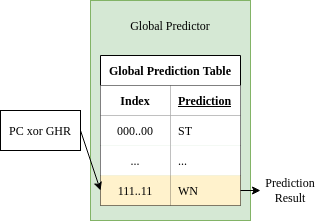
\includegraphics[width=0.3\textwidth]{imgs/global_predictor}
    \caption{The global prediction table is indexed using the xoring result between the program counter and
    the global history register. The prediction result is a 2-bit states which is the same as the prediction
    table used in our local predictor.}
    \label{fig:global_predictor}
\end{figure}

To update the global predictor, we update the corresponding state toward the strongly taken if the outcome is taken,
or update it toward the strongly not-taken in the opposite case. After the state was updated,
we update the global history by left shifting it and add new outcome to the last bit.

\subsection{Predictor chooser}

The predictor chooser is implemented in almost same way as the global branch predictor. The difference is that the chooser
use the instruction address from the program counter as the index, and the 2-bit states determine the
predictor instead. The state 00, 01, 10 and 11 are for strongly local predictor, weakly local predictor,
weakly global predictor and strongly global predictor respectively. The implementation of the predictor chooser
is illustrated in Figure \ref{fig:global_predictor}.

\begin{figure}[h]
    \centering
    % \vspace{0.2cm}
    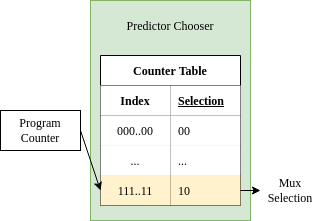
\includegraphics[width=0.3\textwidth]{imgs/predictor_chooser}
    \caption{The predictor chooser is indexed by the address in the program counter. The state in the table
    determines which predictor to use. It acts as a selection bit for the output mux.}
    \label{fig:predictor_chooser}
\end{figure}

The chooser's state will be updated if the output from both predictors are different. We will decrease the
counter state if the local predictor give the correct prediction and the state is not 00. In the other case,
the counter is increased if the state is not 11.

\subsection{Predictor Initialization}

For the local predictor, the local history table was initialize to all not-taken at every
index. Moreover, we set the state for each row in the local prediction table to weakly not-taken
state (01).

In the case of the global predictor, the global history register was also initialized to all not-taken.
The state in each row is also set to weakly not-taken (01) in the global prediction table.

Lastly, we set the predictor chooser's state to 10 which weakly chooses the global predictor
at start for every row in the counter table.

\subsection{Storage analysis}

In this project, we have $64K + 256$ bits to store required informtion in the proposed branch
predictor. This is larger than our baseline which only allow $16K$ bits to store information.
To utilize the larger storage, we increase the number of bits compared to our baseline.

Our GShare baseline use 13 bits to store the global history. While our tournament predictor
utilize 9, 10 and 10 bits to store the global history, the local history and the index for the
local history table respectively. These are due to 16K bits budget limitation of the baseline.

In our approach, we will sepearate half of storage for each predictor. Thus, we used 14 global
history bits for the global predictor. The rest of the storage is used for local predictor with
11 local history bits and 11 address bits. With this information, we can calculate the total
storage used as following.

With 11 bits for both local history and indexing bits, our local predictor used $2^{11} \times 11$
bits for the local history table. Moreover, this means that $2^{11} \times 2$ bits are used for
storing the prediciton table. Thus, total used bits are 26624 bits. 

For the global predictor, we used 14 global history bits. Thus, the size of the prediction
table is $2^{14} \times 2 = 32768$ bits which equals to the total storage for this predictor.

In addition to the predictor, we also have the chooser. We used the same index as the local predictor
to select the chooser. Therefore, the size of the chooser is $2^{11} \times 2 = 4096$ bits.

From these information, the total size of the proposed predictor is
$26624 + 14 + 32768 + 4096 = 63502$ bits which still fit to our budget.

\section{Experimental Setup}

In the project, we experiment the performance of our predictor compared to the given baselines.
Although, baselines have 16K bits limitation. Thus, we have GShare with 13 bits and the tournament
predictor with 9 global history bits, 10 lobal history bits and 10 program counter index bits.
We also extended the this limitation
by exploring the GShare with 15 bits and the tournament predictor with
11 global history bits, 12 local history bits and 12 program counter index bits.
This help show how our predictor preform if our baselines have the same storage budget.

In the testing phase, we have 3 different groups of traces including fp, int and mm.
Each trace group have 2 differnt traces, so there are 6 traces in total. We will run
each predictor with each trace and measure the misprediction rate. A predictor with a lower misprediction rate
means that the performance of it is better.

\section{Observation}

After the experiment was performed and the misprediction rate was collected, we look
further into the result we got.

First, we will look at the performance of our baselines. We will represent the
GShare with $x$ global history bits as GShare:$x$, and the tournament predictor
with $x$ global hisotyr bits, $y$ local history bits and $z$ address index bits
as tournament:$x$:$y$:$z$. The performance of baselines is shown in Table \ref{table:baseline_performance}.

\begin{scriptsize}
\begin{table}[h!]
  \centering
  \caption{Misprediction rate for our baseline predictors with each trace}
  \label{table:baseline_performance}
  \begin{tabular}{|l|l|l|l|l|l|l|}
    \hline
    \textbf{Predictor} & \textbf{fp1} & \textbf{fp2} & \textbf{int1} &\textbf{int2} & \textbf{mm1} & \textbf{mm2}\\
    \hline
    \hline
    GShare:13 & 0.825 & 1.678 & 13.839 & 0.420 & 6.696 & 10.138 \\
    (baseline) & & & & & & \\
    \hline
    GShare:15 & 0.827 & 0.985 & 11.220 & 0.364 & 4.441 & 8.039 \\
    \hline
    Tournament & & & & & & \\
    :9:10:10 & 0.991 & 3.246 & 12.622 & 0.426 & 2.581 & 8.483 \\
    (baseline) & & & & & & \\
    \hline
    Tournament & 0.990 & 0.410 & 10.171 & 0.333 & 1.072 & 6.967 \\
    :11:12:12 & & & & & & \\
    \hline
  \end{tabular}
\end{table}
\end{scriptsize}

Regarding the Table \ref{table:baseline_performance}, we can see that GShare baseline is better than
the tournament baseline for fp trace group. This infers that fp traces involves a lot of branches that have
global correlation. In the other hand, the tournament
baseline is better if we consider mm trace group. One reason is that the tournament predictor can handle
local branch correlations while GShare cannot. Thus, it has better performance on this trace group.
Both predictors performed
great on int trace group. Moreover, although these predictors are extended
to larger storage budget, none of these perform better than both original baselines
at every traces. The tournament:11:12:12 might look promising, as it can beat 11 out of 12
baseline traces. However, it didn't pass the requirement of the project. That's why we came up
with our proposed method. Especially for trace fp1, we believe that using xor result
between the program counter and the global history register for the global predictor
is the key to beat this trace.

After we implemented our proposed method, we get the result as shown in the Table \ref{table:our_performance}.
Misprediction rates of our predictor is lower than both baselines for all 6 traces (total 12 traces win).
Our predictors is also better than tournament:11:12:12 for 4 out of 6 traces. Moreover,
it outperformed GShare:15 for all traces. From these result, this means that our predictor
can perform very promising prediction for both local and global branch correlation compared
to other methods.

\begin{scriptsize}
\begin{table}[h!]
  \centering
  \caption{Misprediction rate for our method with each trace}
  \label{table:our_performance}
  \begin{tabular}{|l|l|}
    \hline
    \textbf{Trace} & \textbf{Misprediction Rate}\\
    \hline
    \hline
    fp1 & 0.811 \\
    \hline
    fp2 & 0.244 \\
    \hline
    int1 & 10.294 \\
    \hline
    int2 & 0.281 \\
    \hline
    mm1 & 1.880 \\
    \hline
    mm2 & 6.550 \\
    \hline
  \end{tabular}
\end{table}
\end{scriptsize}
\section{Results}

From previous section, our predictor outperformed both baselines predictor
for all traces. It showed that it can solve indexing collision problem which we encountered
in fp1 trace which is a problem in the tournament predictor. Moreover, the
misprediction rate of our predictor showed that it can handle both local and global
branch correlations. The summary of the result for the proposed method and baselines
are shown in Table \ref{table:result}.

\begin{scriptsize}
\begin{table}[h!]
  \centering
  \caption{Final misprediction rate results for baselines and our method for each trace.}
  \label{table:result}
  \begin{tabular}{|l|l|l|l|l|l|l|}
    \hline
    \textbf{Predictor} & \textbf{fp1} & \textbf{fp2} & \textbf{int1} &\textbf{int2} & \textbf{mm1} & \textbf{mm2}\\
    \hline
    \hline
    GShare:13 & 0.825 & 1.678 & 13.839 & 0.420 & 6.696 & 10.138 \\
    \hline
    Tournament & & & & & & \\
    :9:10:10 & 0.991 & 3.246 & 12.622 & 0.426 & 2.581 & 8.483 \\
    \hline
    \hline
    \textbf{Our predictor} & \textbf{0.811} & \textbf{0.244} & \textbf{10.294} & \textbf{0.281} & \textbf{1.880} & \textbf{6.550} \\
    \hline
  \end{tabular}
\end{table}
\end{scriptsize}

\section{Conclusion}

In this work, we proposed a branch predictor method which is based on Alpha 21264's tournament predictor.
We update index hashing for the global predictor to use xor result between the program counter and the global
history register as in GShare to solve index collision problem. We also changed the index of the predictor chooser
to use the program counter. The predictor was config to use 14 global history bits,
11 local history bits and 11 address index bits. The total storage used is 63502 bits which fit in our requirement.
The proposed predictor was benchmarked with 6 different address traces, and it is compared to
GShare with 13 global history bits and the tournament predictor with 9 global history bits, 10 local history bits
and 10 address index bits. The result showed that our predictor outperformed the requirement baselines
by great amount of margin for all address traces.

\section*{Acknowledgements}
This work is done alone so I don't have any teammates. Thanks the professor and TAs for good materials in this
courses. Most of the knowledge that I used to finished this project is from course slides.

%%%%%%% -- PAPER CONTENT ENDS -- %%%%%%%%


%%%%%%%%% -- BIB STYLE AND FILE -- %%%%%%%%
\bibliographystyle{IEEEtranS}
\bibliography{refs}
%%%%%%%%%%%%%%%%%%%%%%%%%%%%%%%%%%%%

\end{document}

